\documentclass[12pt,a4paper]{cibb}

\usepackage{subfigure,graphicx}
\usepackage{amsmath,amsfonts,latexsym,amssymb,euscript,xr}
\usepackage{booktabs}
\usepackage[nodayofweek]{datetime}
\usepackage{hyperref}

\usepackage[table]{xcolor}
\usepackage{color,colortbl,tabularx}

\usepackage[english]{babel}
\usepackage[protrusion=true,expansion=true]{microtype}
\usepackage{amsmath,amsfonts,amsthm}
% \usepackage[pdftex]{graphicx}
% \usepackage{pifont}

\def\red{\color{red}}
\def\black{\color{black}}
\def\blue{\color{blue}}
\def\magenta{\color{magenta}}

\definecolor{LightBlue}{rgb}{0.88,0.9,0.9}


\title{\large $\ $\\ \bf Product and Store Level Sales Forecasting for Retail} 

% \author{ Vivek Dhullipala, Juwon Lee, Prathmesh Savale,  Bolun Zhang }



\abstract{
{\bf Abstract.} The goal of this project is to create sales forecasts for Favorita stores in Ecuador. We are given the day level sales data of 33 product families across 54 stores from 2013 - 2017. It also includes information of holidays and promotions. Overall, the question to be answered is - can sales of different product families selling across multiple stores be predicted through historical data?}

\begin{document}
\thispagestyle{myheadings}
\pagestyle{myheadings}
\markright{\tt MIS S381N: Group(16) Project Report, Summer 2022}



\section{\bf Importance of the Issue}
\label{sec:IMPORTANCE-OF-ISSUE}
A good forecasting model will allow the stores to accurately predict and control inventory leading to less waste of perishable goods, higher revenues, and greater customer satisfaction. An accurate forecast can also help the finance department plan their budget and buyers plan their purchase.


\section{\bf Exploratory Data Analysis}
\label{sec:EDA}

\subsection{\bf \it Time series trends across stores}
We looked at the entire training dataset~\cite{kaggledataset}  on an aggregated level based on stores. As demonstrated in the time series plot below, the majority of the 54 stores’ sales moves in a strong correlation across time. Additionally, there are large spikes of sales near the end of years each year suggesting that the holidays such as Christmas affect the overall sales across all the stores. 

\subsection{\bf \it Time series trends across product families}
For each of the 33 families we plot the sales across time. Similar to stores the products do not show much variation in their time series shapes. Overall, the families that had the most sales were GROCERY I, BEVERAGES,  CLEANING, BREAD/BAKERY, and DAIRY. Overall, these are products that people will buy year-round. They are also products that are price-inelastic meaning that a customer’s demand for the product will not change based on price changes.

\begin{figure}[h]
\hfill
\subfigure[Sales across stores]{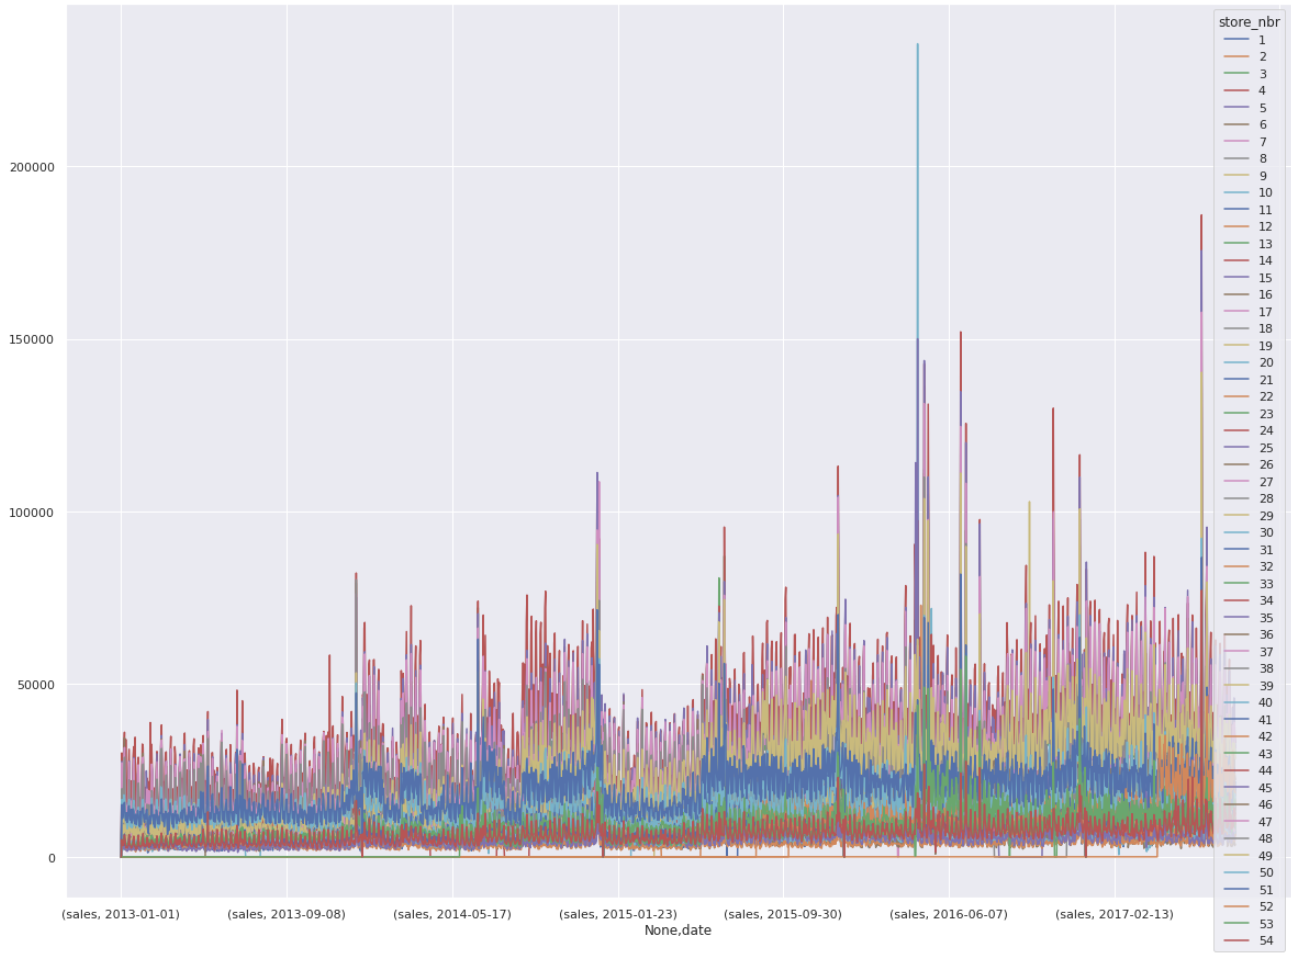
\includegraphics[width=7cm]{store_sales.png}}
\hfill
\subfigure[Sales across product families]{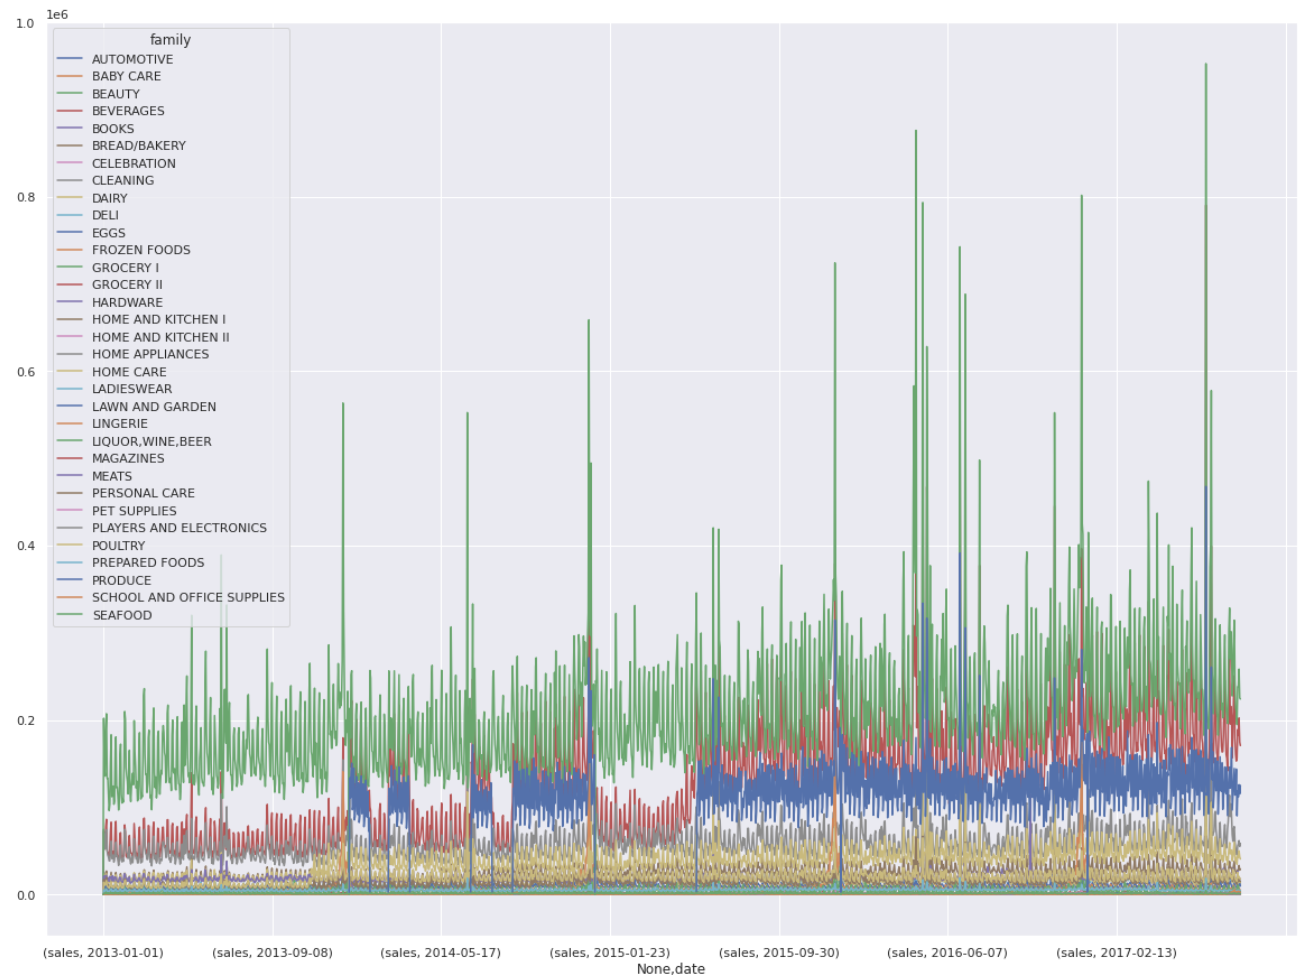
\includegraphics[width=7cm]{product_sales.png}}
\hfill
\caption{Time series trends across stores and product families}
\end{figure}

For both product families and stores we used dynamic time warping to cluster similar time series shapes. But since majority of the time series have the same shape, we do not see the any variation in the clusters.

\subsection{\bf \it Impact of external factors (holiday and promotions) on sales}
We do a univariate analysis of sales vs. external factors like holiday and promotions and see that there is a slight impact of such regressors on the overall sales. These external factors will be useful in modeling.

\begin{figure}[h]
\hfill
\subfigure[Sales vs. Holidays]{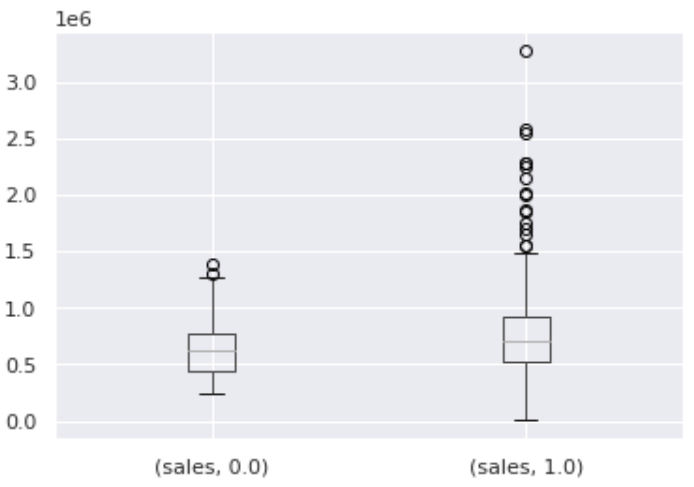
\includegraphics[width=7cm]{sales_v_holiday.png}}
\hfill
\subfigure[Sales vs. Promotions]{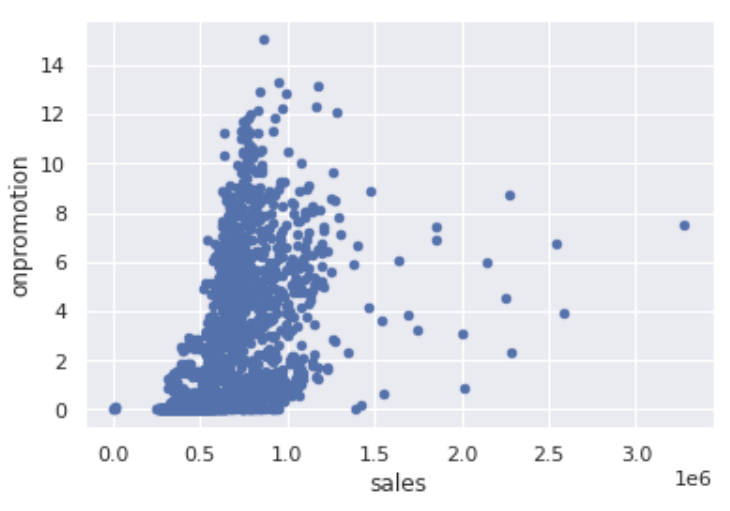
\includegraphics[width=7cm]{sales_v_promotions.png}}
\hfill
\caption{Impact of holidays and promotions on Sales}
\end{figure}

\subsection{\bf \it Impact of oil on sales}
Oil prices have a strong negative correlation with sales. So with a decrease in oil prices the sales tend to go up.

\begin{figure}[h]
 \begin{center}
{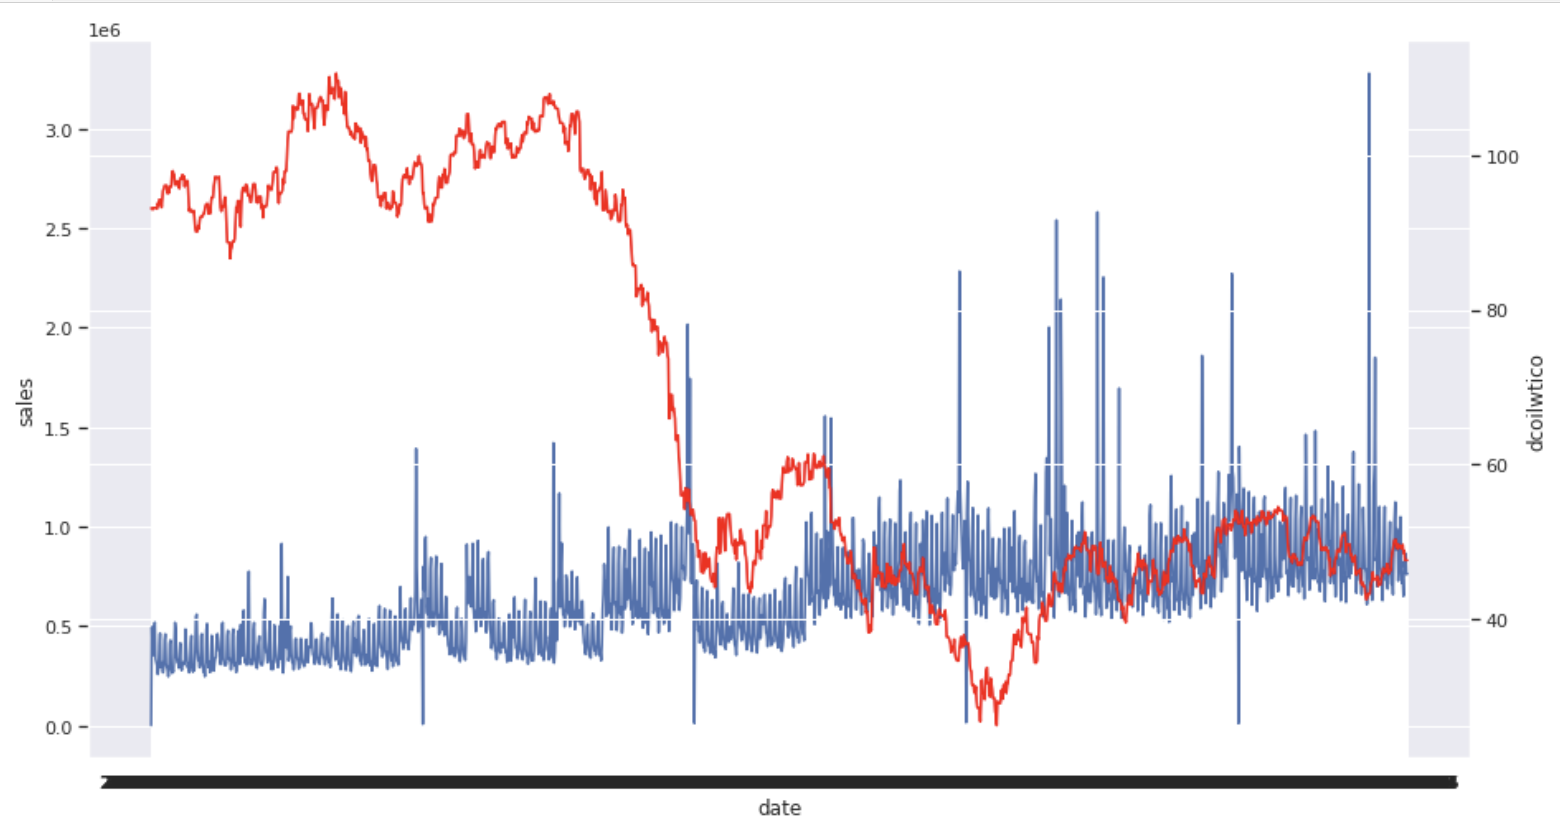
\includegraphics[width=10cm]{sales_v_oil.png}}
\caption{Impact of oil on sales}
 \end{center}
\end{figure}

\section{\bf Modeling}
\label{sec:MODELING}
We followed a 3 step approach for forecasting sales at and overall level and product store level.

\subsection{\bf \it Decompose the time series}
We decompose the time series into trend, seasonal and irregular components using the statsmodels package in python. Statsmodels uses a centered moving average to calculate the trend. The trend is then subtracted from the original time series and the leftover part is averaged across the specific time periods to get the seasonality. The calculated trend and seasonality is then removed the original time series to get the residual/irregular component.

\begin{figure}[h]
\vspace{3mm}
 \begin{center}
{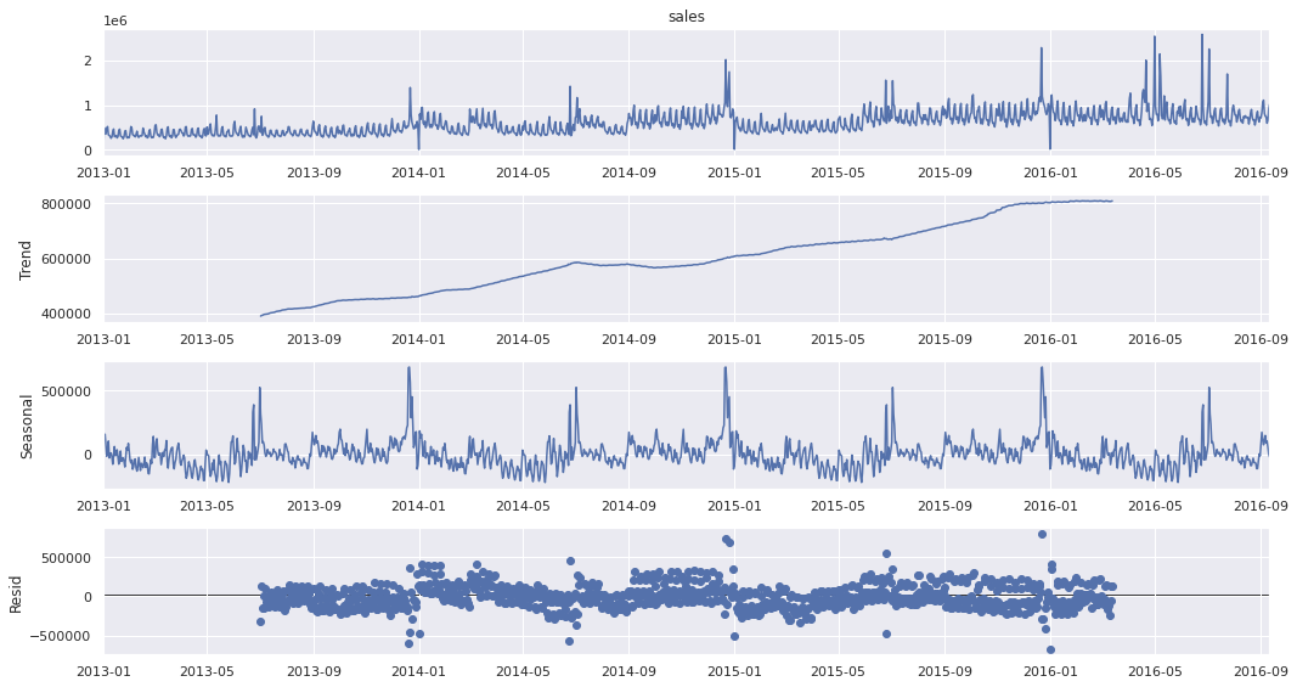
\includegraphics[width=10cm]{stl_decomposition.png}}
\caption{Decomposing time series to trend, seasonal and irregular}
 \end{center}
 \vspace{-8mm}
\end{figure}

\subsection{\bf \it Remove effect of external regressors from residual}
We calculate the beta estimates for the OLS fit of external regressors vs. residuals. This helps gauge impact of the regressors like holiday and promotions on the residue. Since holidays and promotions are random, they are not captured in the seasonal component and they cannot be modelled, therefore their effect needs to be removed from the residue before it is modelled.  

\subsection{\bf \it Model residual}
The adjusted residual component can be modelled after the random impact has been removed. There are multiple techniques to do this, we have experimented with an ARIMA(0,0,0) and a random walk ARIMA(0,1,0) model. This gives us the required improvement over baselines forecast results using prophet without tuning.

\subsection{\bf \it Add effect of external regressors back to residual}
Since the residue has been modeled without the effect of external regressors. We add their effect back using the initially calculated beta values.

\subsection{\bf \it Forecast by extrapolating trend, seasonality and adding adjusted residual}
The extrapolated trend, seasonality and adjusted residual component are added back to get the required forecast.

\begin{figure}[h]
\vspace{3mm}
 \begin{center}
{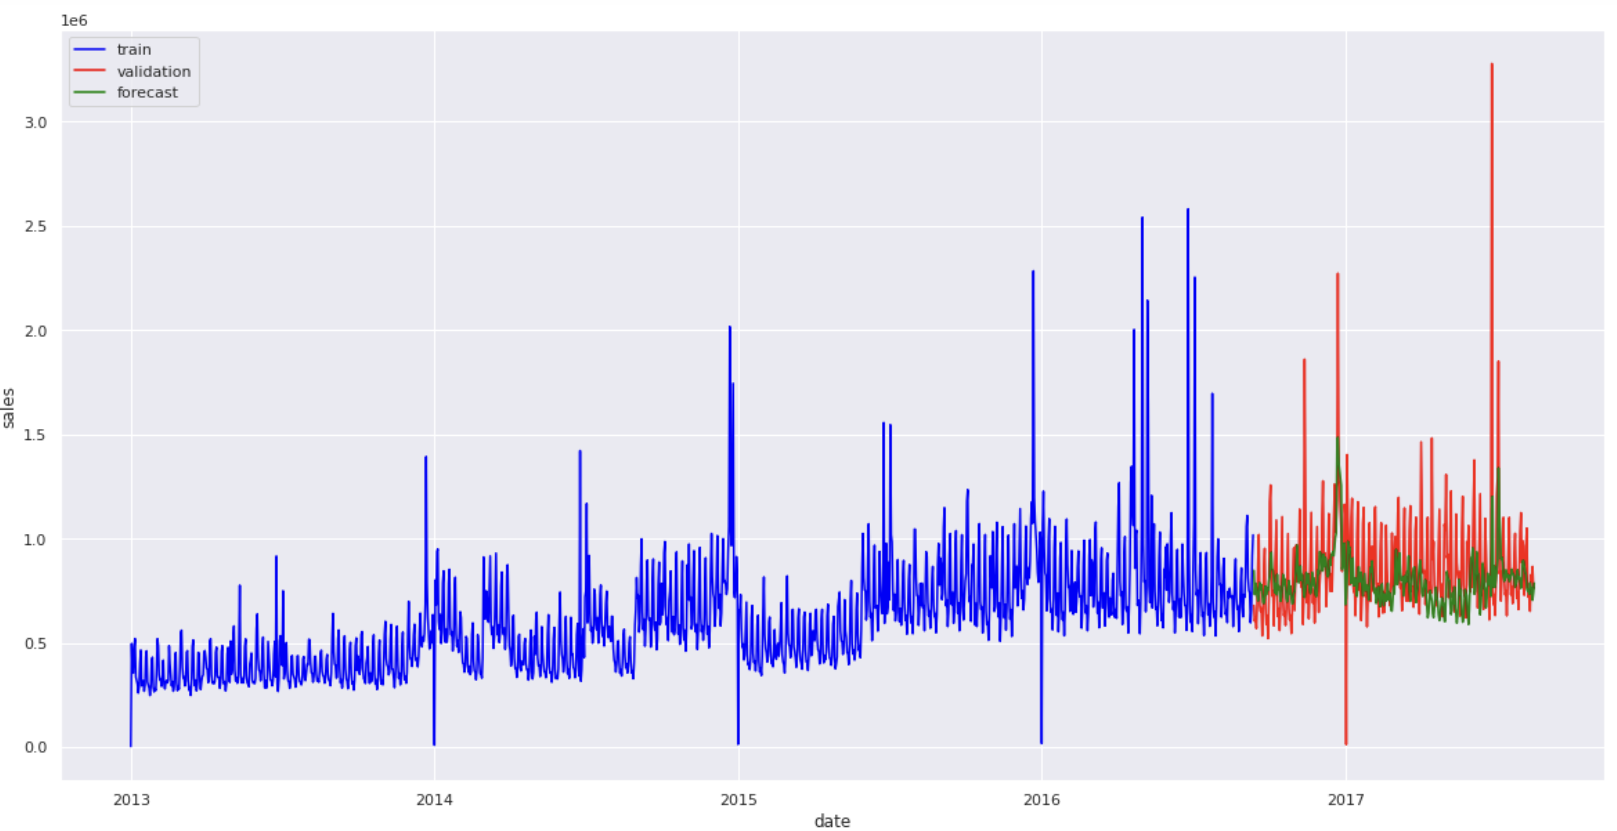
\includegraphics[width=10cm]{forecast_result_stl.png}}
\caption{Forecast result with STL decomposition and adjustment for external regressors}
 \end{center}
 \vspace{-8mm}
\end{figure}


\section{\bf Results}
\label{sec:RESULTS}
We use pyspark to scale this framework across multiple stores and products. We observe the following results.


\begin{table}[httb!] \small
\centering
    \begin{tabularx}{0.8\textwidth}{ l  l  c }
        \toprule
          \textbf{method} & \textbf{MAE} & \textbf{runtime} \\
        \midrule
        \rowcolor{LightBlue} STL decompose & 139.24 & 34 sec \\
         STL decompose + residue adjust & 135.25 & 58 sec \\
        \rowcolor{LightBlue}  fbprophet & 148.47 & 6min 2sec\\
        \bottomrule
    \end{tabularx}
    \caption{
    Average mean absolute error results across 3 iterations for store and product level dataset\label{tab:RESULTS}}
\end{table}




\section{\bf Conclusion}
\label{sec:CONCLUSIONS}

STL decomposition with trend and seasonality extrapolation and STL decomposition with residue adjustment give satisfactory results. They have simple implementation and are easy to interpret and explain. On the other hand Auto-ML techniques like prophet take more time for execution, cost compute resources and are black box making the results difficult to interpret.

\footnotesize
\bibliographystyle{unsrt}
\bibliography{bibliography_CIBB_file.bib} 
\normalsize



\end{document}



